\documentclass[a4 paper]{article}
\usepackage[T1]{fontenc}
\usepackage[utf8]{inputenc}
\usepackage{amsmath}
\usepackage{amssymb}
\usepackage{hyperref}
\usepackage{parskip} %skip the indent of a new paragraph.
\usepackage{float}
\usepackage{graphicx}
\usepackage{listings}
\usepackage[per-mode=symbol]{siunitx}
\usepackage{epstopdf}
\usepackage[super]{nth}
\usepackage[toc,page]{appendix}
\usepackage{enumerate}
\usepackage{verbatim}
\usepackage[ruled, vlined, linesnumbered]{algorithm2e}
\usepackage{mathtools}
\usepackage{gensymb}
\usepackage{textcomp}
\usepackage{pdfpages}
%\lstset{language=Matlab, frame=single, breaklines=true,numbers=left, keywordstyle=\color{blue},rulecolor=\color{black},commentstyle=\color{gray}}

\usepackage{cleveref}
\usepackage[]{todonotes}

%% Brukes for tabeller (av likninger)
\usepackage{tabularx}
\def\tabularxcolumn#1{m{#1}}

\newcommand{\mbf}[1]{\mathbf[#1]}
\newcommand{\partialderiv}[2]{\frac{\partial{#1}}{\partial{#2}}} % prints partial derivative as a fraction

\DeclareUnicodeCharacter{2212}{-} % Needed to import matplolib figures without trouble

\begin{document}
    \section{Funksjonell beskrivelse av hele systemet.}

Systemet skal implementere en temperatur-regulator, som skal kontrolere
meskeprossessen som er en del av ølbryggingsprosessen. Temperaturen skal måles
med en DS18S20 onewire digital temperatursensor. Og styres ved hjelp av to
relèer som kan hendholdsvis øke og minke pådraget til en Caso pro 3500
induksjonskokeplate. Systemet skal kunne følge en tidsserie av referanser
(f.eks. 60\textdegree{} i 30min, 65\textdegree{} i 20min, ...), og logføre referanse,
temperatur og pådrag. Det skal være mulig å kontrolere systemet samt hente
logger og nåverdier over internett. Se neste side for ett kontekstdiagram av hele 
systemet.

\newpage
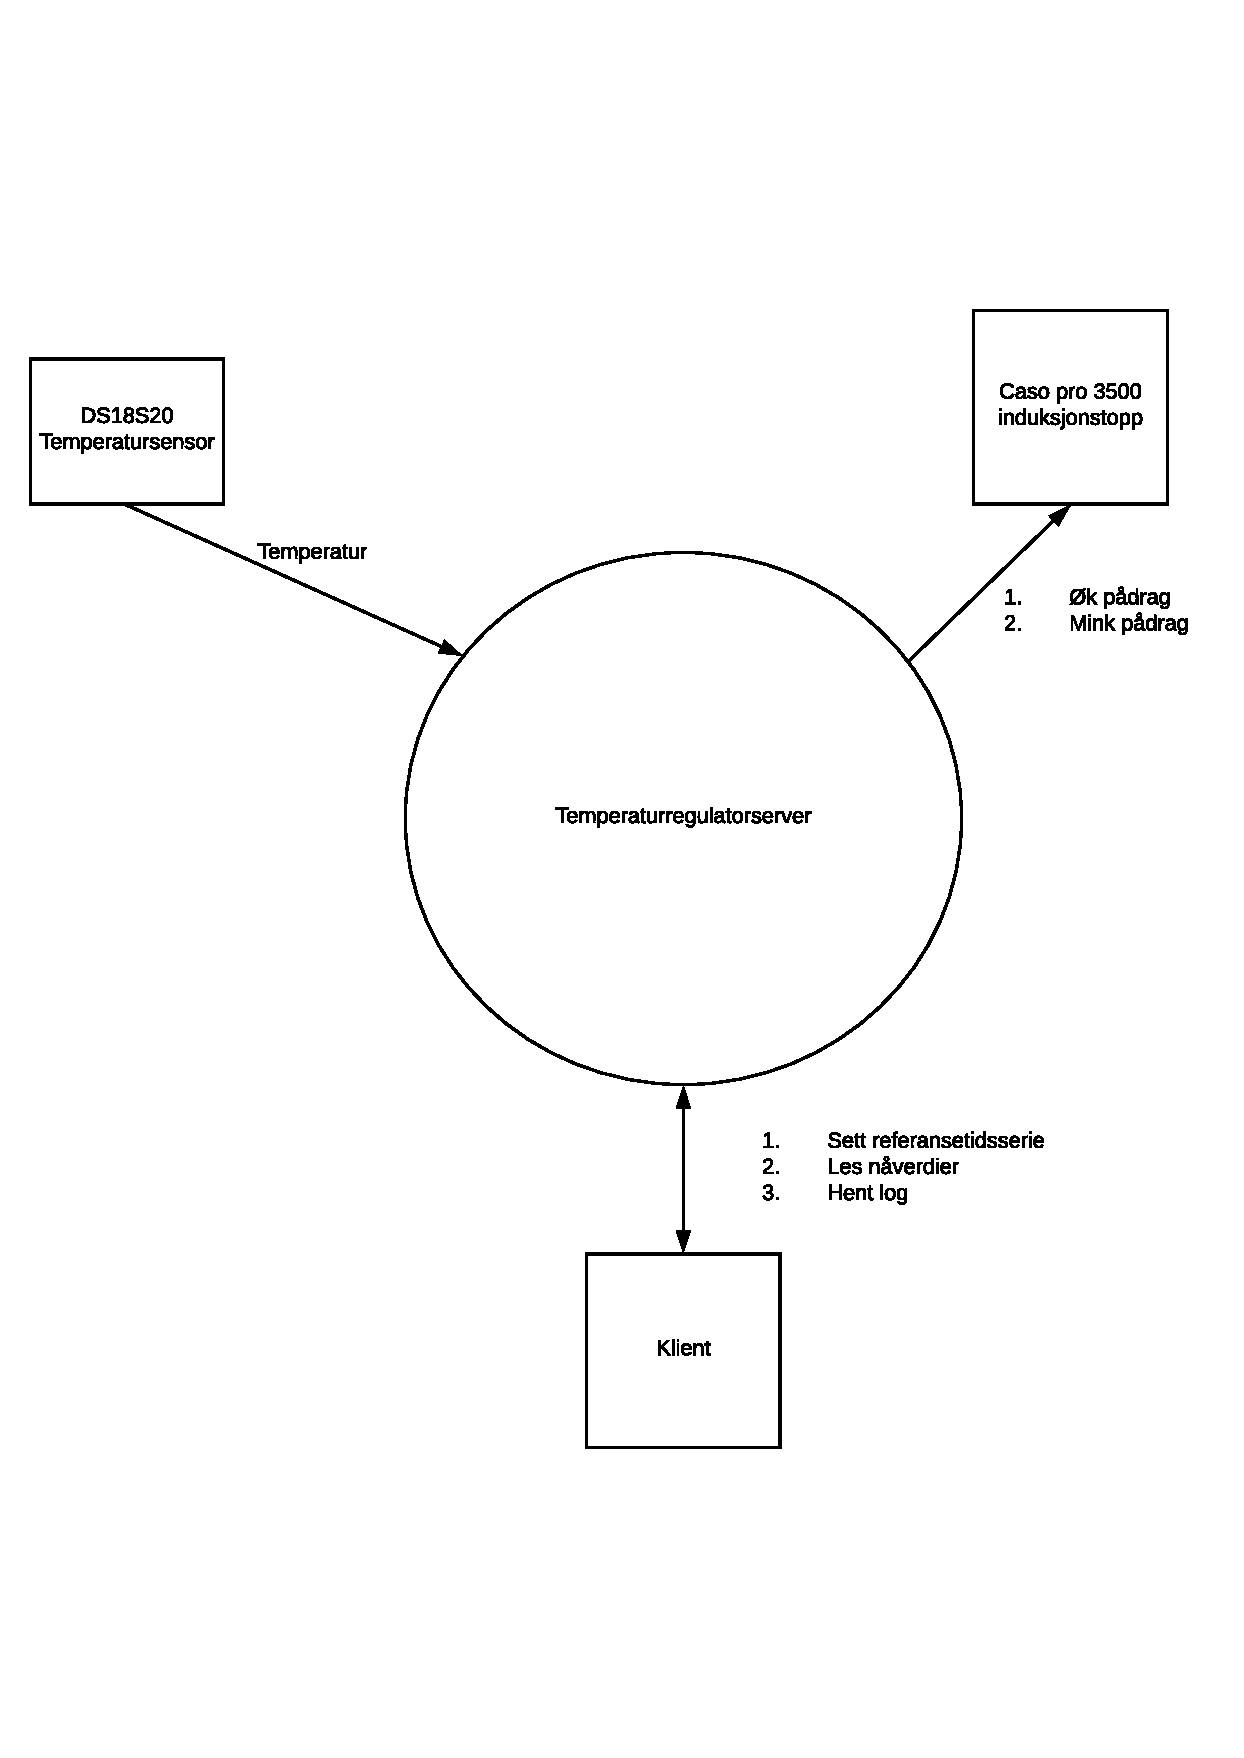
\includepdf[pages={1}]{context_diagram.pdf}
\newpage

\section{Modularisering}
Systemet kan deles opp i 3 moduler. En regulatormodul som tar seg av alt av
lesing av sensorer, selve reguleringen og setting av pådrag; en webserver-modul
som håndterer all kommunikasjon med klienten; og en logger-modul som
logger det regulatoren gjør, og kan levere disse loggene til webserver-modulen.

Webserver-modulen er ansvarlig for all kommunikasjon med klienten. Den må kunne
motta en tidsserie som kan bli brukt av regulatoren som referanse. I tillegg må
webserveren kunne levere de siste målte og satte verdiene, i tillegg til å kunne
levere logger over hele tidsforløpet til en prosess.

Regulator-modulen skal kunne regulere temperaturen målt med en temperatursensor
til å følge temperaturen bestemt av tidsserien den mottar fra webserver-modulen.
Dette gjøres med en PID-regulator som styrer pådraget til ett varmeelement. Den
målte verdien, sammen med referanse og pådrag skal sendes til logger-modulen
slik at det senere er mulig å se hvordan temperaturforløpet var.

Logger-modulen mottar verdier fra regulator-modulen, og lagrer dem på en
permanent måte, slik at det senere er mulig å hente ut loggen som tilhører en
bestemt tidsserie. Loggen som hentes ut skal være på ett format som gjør det
lett å lage en graf basert på loggen.

En oversikt over hvordan de ulike modulene kommuniserer med hverandre og
omverden kan sees på neste side.

\newpage
\includepdf[pages={2}]{context_diagram.pdf}

\end{document}
